\documentclass[10pt,prd,aps,a4paper,twocolumn,superscriptaddress,nofootinbib,floatfix]{revtex4-2}
\pdfoutput=1

\usepackage[T1]{fontenc}
\usepackage[utf8]{inputenc}
\usepackage{lmodern}

\usepackage{amsmath,amssymb,amsfonts,bm,mathrsfs}

\usepackage{graphicx}
\usepackage{booktabs}
\usepackage{dcolumn}

\usepackage{color}

\makeatletter
\newcommand{\adddotsbeforeeqnnum}{%
    \renewcommand{\theequation}{\arabic{equation}.}%
}
\makeatother

\usepackage{braket}

\usepackage[linktoc=none]{hyperref}
\hypersetup{colorlinks,			
	linkcolor=blue,
	citecolor=blue}

\begin{document}

\title{Reconstruction of Black Hole Ringdown Signals with Data Gaps using a Deep-Learning Framework}
\author{Jing-Qi Lai}\email{laijingqi19@mails.ucas.ac.cn}
\affiliation{School of Physical Sciences, University of Chinese Academy of Sciences, Beijing 100049, China}
\author{Jia-Geng Jiao}\email{jiaojiageng@ucas.ac.cn}
\affiliation{International Centre for Theoretical Physics Asia-Pacific,
University of Chinese Academy of Sciences, Beijing 100190, China
}
\author{Cai-Ying Shao}\email{shaocaiying@ucas.ac.cn}
\affiliation{School of Physical Sciences, University of Chinese Academy of Sciences, Beijing 100049, China}

\author{Jun-Xi Shi}\email{shijunxi23@mails.ucas.ac.cn}
\affiliation{International Centre for Theoretical Physics Asia-Pacific,
University of Chinese Academy of Sciences, Beijing 100190, China
}
\author{Yu Tian}\email{ytian@ucas.ac.cn}
\affiliation{School of Physical Sciences, University of Chinese Academy of Sciences, Beijing 100049, China}
\affiliation{Institute of Theoretical Physics, Chinese Academy of Sciences, Beijing 100190, China}

\begin{abstract}
Data gaps can obscure the rapidly decaying oscillations of a black hole ringdown, making its phase and decay envelope difficult to recover. We present DenoiseGapFiller (DGF), a deep-learning framework for joint denoising and waveform reconstruction. Its dual-branch encoder combines local time--frequency features with multiscale temporal context, allowing information on both sides of a gap to guide reconstruction. A waveform decoder and mask-aware residual blocks turn the fused representation into a complete signal estimate. We test the framework on independent simulated LISA A/E signals with suppression intervals spanning approximately 6\%--10\% of the analysis window. DGF achieves a mean noise-weighted mismatch of $8.52\times10^{-3}$ across the test population and $5.32\times10^{-3}$ for signals with network signal-to-noise ratio $\rho\ge10$. The reconstructed waveforms recover the phase at the signal-envelope peak with mean absolute errors below $4^\circ$ in both channels. This recovery of waveform shape and peak phase supports DGF as a reconstruction tool for ringdown studies under the stated simulation assumptions.
\end{abstract}

\maketitle
\section{Introduction}
The ringdown following a binary black hole merger carries information about the remnant spacetime. In the perturbative regime, its waveform is described by damped quasinormal modes whose frequencies and decay times depend on the mass and spin of a Kerr black hole~\cite{berti2006gravitational,berti2009qnm}. Measuring these modes is the basis of black hole spectroscopy and ringdown tests of general relativity~\cite{Isi_2019}. Space-based observatories such as LISA, Taiji and TianQin offer access to the ringdowns of massive black hole binaries in the millihertz band~\cite{amaroseoane2017laserinterferometerspaceantenna,robson2019construction,Ruan2020,Luo2016}.

Ringdown amplitudes decay rapidly. An interruption near the onset can therefore remove a substantial fraction of the signal even when its duration is short compared with the analysis window. Scheduled interruptions and unscheduled data losses are relevant to space-based observations~\cite{Baghi2019,dey2021gaps}. Shi \textit{et al.}~\cite{shi2024effectsdatagapsringdown} examined their effects on ringdown observability and parameter estimation. Multiplication by a gap window also redistributes power across Fourier frequencies~\cite{Harris1978}. The reconstruction problem consequently concerns the phase and decay envelope across the gap, as well as the complete waveform. An interval covering 20\% of a short record illustrates a severe interruption; the variable-duration LISA protocol considered here covers approximately 6\%--10\% of a 528-s record.

Existing approaches exploit different information about the missing signal. Interpolation uses neighboring samples, with accuracy determined by the bandwidth, sampling and interpolation rule~\cite{Horowitz1974,Maeland1988,Unser1999}. Bayesian data augmentation treats missing samples as latent variables in source-parameter inference~\cite{Baghi2019}. Sparse inpainting exploits structure in Fourier or wavelet representations and has been applied to LISA galactic-binary signals~\cite{Blelly2021,Starck2010}. Learned dictionaries provide another way to encode waveform structure for denoising~\cite{TorresForne2016}. Ringdown reconstruction poses a specific challenge for these approaches: the waveform is oscillatory, its envelope changes rapidly, and the available context can be strongly asymmetric about the gap.

Neural methods learn reconstruction maps from simulated waveforms and noisy observations. Xu \textit{et al.}~\cite{Xu_2024} used a DenseNet--BiLSTM model for inspiral--merger--ringdown signals under several forms of corruption. Mao \textit{et al.}~\cite{Mao:2025cae} combined a convolutional autoencoder with a bidirectional gated recurrent unit for long LISA sequences containing gaps. WaveFormer~\cite{Wang:2024waveformer} combines convolutional feature extraction and Transformer blocks for denoising ground-based data, and assesses amplitude and phase recovery separately. These studies motivate learned waveform estimation. Their waveform families, detector responses and noise conditions also define the domains in which their reported performance applies.

We develop DGF to recover damped oscillations from noisy observations with a known gap. The time--frequency branch represents local oscillatory content through complex Morlet coefficients. The temporal branch preserves the sign and multiscale structure of the waveform. Mixing layers combine these complementary features, and sequence blocks connect context on both sides of the interval before a decoder synthesizes the clean waveform. Related time-series models use temporal and feature mixing to combine information across scales~\cite{TSMixer2023,TimeMixer2024}. The LISA configuration incorporates PSD whitening, mask-aware and joint-channel modules, and noise-conditioned coefficients in a signal basis fitted to clean training waveforms.

The observation model is $d=Gh+n$: $G$ suppresses the signal over one interval, and noise is present throughout the record. We assess recovery through direct waveform mismatch, amplitude residuals, error spectra and per-channel analytic phase. Full-population distributions establish the typical accuracy and its upper tail; separate peak-masking statistics resolve the effect of losing the strongest part of the signal. Waveform comparisons show the recovered oscillations across gaps containing the signal-envelope peak. All reconstruction results use one selected DGF model and the independent LISA test population defined in Sec.~\ref{sec:method}. The source and channel conventions are common to training, validation and testing.

Section~\ref{sec:method} presents the reconstruction framework, signal and noise models, and training protocol. Section~\ref{sec:results} evaluates waveform recovery, gap-location dependence, amplitude fidelity and phase accuracy. Section~\ref{sec:discussion} discusses the implications for ringdown analysis and the scope of the simulations. The appendixes provide implementation details, additional waveform diagnostics and tests with fixed gap durations.

\section{Methodology}\label{sec:method}
We generate simulated ringdown observations using standard LISA response and noise models. DGF operates on the $A/E$ TDI channels and estimates their complete clean waveforms from the observations and known gap mask. The signal, response, noise calibration and preprocessing described below are shared by the training, validation and independent test sets.

\subsection{Physical ringdown signals and LISA response}\label{sec:physical_signals}
The source population consists of nonspinning progenitor binaries. The source-frame total mass $M_{\rm tot}^{\rm src}$ is drawn log-uniformly from $10^5$ to $5\times10^6\,M_\odot$, the light-to-heavy mass ratio $q=m_2/m_1$ uniformly from $0.3$ to $1$, and redshift $z$ uniformly from $1$ to $6$. Sky position and inclination are isotropic; polarization and orbital phase are uniform on their angular ranges. We use a flat $\Lambda$CDM distance relation with $H_0=67.4\,\mathrm{km\,s^{-1}\,Mpc^{-1}}$ and $\Omega_m=0.315$.

The SEOBNRv4 remnant prescription implemented in LALSimulation determines the source-frame remnant mass $M_f^{\rm src}$ and dimensionless spin $\chi_f$. The Kerr-mode frequencies and damping times use the detector-frame remnant mass,
\begin{equation}
M_f^{\rm det}=(1+z)M_f^{\rm src}.
\end{equation}
The fundamental modes $(\ell,m,n)=(2,2,0),(2,1,0),(3,3,0),(4,4,0)$ enter the PyCBC time-domain ringdown generator~\cite{berti2006gravitational,berti2009qnm,PyCBCRingdown}. Spherical angular harmonics and luminosity-distance scaling specify the polarizations. Writing $q_\star=1/q$, the mode excitation coefficients are~\cite{Kamaretsos2012}
\begin{align}
\alpha_{22}&=0.25e^{-q_\star/7.5},\nonumber\\
\frac{\alpha_{21}}{\alpha_{22}}&=0.13(q_\star-1)^{1/2},\qquad
\frac{\alpha_{33}}{\alpha_{22}}=0.18(q_\star-1)^{1/3},\nonumber\\
\frac{\alpha_{44}}{\alpha_{22}}&=0.024q_\star^{3/4}.
\end{align}
These fits refer to the reference epoch used by Kamaretsos \textit{et al.}, ten remnant-mass time units after the dominant-mode luminosity peak. The relative phase convention is $\phi_{\ell m}=m\phi_{\rm orb}$. It defines a simplified coherent mode family for this reconstruction study. PyCBC's pre-reference exponential ring-up joins continuously to the damped-mode segment, whose excitation normalization is retained. The envelope has different one-sided slopes at the reference time. This onset convention and the delayed TDI combinations are retained in the reconstruction targets.

The polarizations are projected onto the constellation links with \texttt{fastlisaresponse}~\cite{Katz2022Response}. Delayed link combinations produce second-generation TDI $X,Y,Z$ observables in an idealized equal-arm constellation. The analyzed channels are
\begin{equation}
A=\frac{Z-X}{\sqrt{2}},\qquad E=\frac{X-2Y+Z}{\sqrt{6}}.\label{eq:aet_convention}
\end{equation}
Both channels are expressed in fractional-frequency units. We generate the response on a padded parent sequence, remove the padding and select a 528-s analysis window. Reconstruction is evaluated on that finite window, including for signals whose damping times exceed its duration.

\subsection{Instrument noise, calibration and whitening}\label{noise model}
Independent stationary Gaussian $A/E$ instrument-noise realizations are generated from the second-generation TDI sensitivities provided by LISA Analysis Tools, with the \texttt{scirdv1} instrument model and no confusion foreground~\cite{LISAAnalysisTools}. For an interior real-FFT bin, the independent real and imaginary noise quadratures have variance $N_p f_s S_c(f_k)/4$, where $N_p$ is the padded parent length and $c\in\{A,E\}$. The inverse transform and padding removal give the simulated time series.

A fixed PSD $S_{c,\rm cal}(f_k)$ is estimated by averaging one-sided periodograms from 512 independent noise-only segments, each containing $N=1056$ samples at $f_s=2\,\mathrm{Hz}$. Estimating the PSD after cropping accounts for finite-window leakage near transfer-function nulls. The same calibration arrays define whitening, the training loss and the comparison metric for every model. The metric weights Fourier bins diagonally; likelihood calculations must also account for correlations introduced by the finite window.

The observation is whitened by the invertible transformation
\begin{equation}
u_c=W_cd_c=\operatorname{irfft}\!\left[
\frac{\operatorname{rfft}(d_c)_k}{\sqrt{f_sS_{c,\rm cal}(f_k)/2}}\right].\label{eq:whitening}
\end{equation}
At DC and Nyquist, positive neighboring-bin values define the whitening factors. Inverse whitening then restores the original fractional-frequency units. These two bins have zero weight in the primary overlap. The first 128 calibration segments determine the expected white-noise RMS, excluding DC and Nyquist, for the coefficient head. All calibration segments are independent of the signal population and test observations.

\subsection{Analysis windows and data gaps}\label{sec:gaps}
For each channel we use the observation and binary mask
\begin{equation}
d_{c,j}=G_jh_{c,j}+n_{c,j},\qquad m_j=1-G_j,\label{eq:observation}
\end{equation}
where $G_j=0$ inside the gap and $G_j=1$ elsewhere. The supervised target is the complete clean $A/E$ waveform $h_{c,j}$. Instrument noise remains present inside the interval. Masking is applied to the physical signal before whitening.

Gap widths are sampled uniformly from the 21 even integers $64,66,\ldots,104$, corresponding to 32--52 s or 6.06\%--9.85\% of the record. Changing the width preserves the reference interval center. Fixed widths of 66 and 100 samples provide additional duration checks. The parent response peak sets the event-centered simulation window, with reference gap offsets drawn between $-66$ and $66$ s. A second seeded draw places the reference interval start at local samples 132--263 and determines the crop. The network receives the resulting observation and known mask at inference.

\subsection{Dual-branch DGF encoder and waveform synthesis}\label{sec:architecture}
Figure~\ref{fig:architecture} shows the DGF architecture. The two $A/E$ channels share encoder weights. The time--frequency branch represents a complex Morlet CWT by its modulus and argument. Sixteen scales and a factor-four temporal subsampling give a $2\times16\times264$ array per channel. Mixing along the temporal, feature and scale axes, followed by convolutional embedding and linear projection, produces $8\times32\times64$ features.

A second Morlet CWT uses 16 logarithmically spaced frequencies from $0.002$ to $0.25\,\mathrm{Hz}$. Three convolutional stages with group normalization and GELU map these low-frequency features to an additive correction before the time--frequency branch projection.

The temporal branch subtracts the observed mean, divides by the observed standard deviation and computes a db4 decomposition. Eight reconstructed subbands preserve signed time-domain information. Each is divided into 32 overlapping patches of 64 samples with stride 32, giving the same $8\times32\times64$ feature shape. The relation $1056=64+31\times32$ fixes the input length.

The branch features are added and passed through token, convolutional and sinusoidal position embeddings. A residual Conv2d layer precedes 16 sequence blocks, each containing channel-wise scaled dot-product attention, normalization and a feedforward layer. The decoder maps features to waveform patches, averages overlapping samples, sums the subbands and applies a Conv1d layer. Restoring the observation normalization gives the channel prediction. Appendix~\ref{app:model_analysis} specifies the attention operation and numerical implementation.

\begin{figure*}[t]
\centering\includegraphics[width=\textwidth]{architecture_dgf_20261015.pdf}
\caption{DGF architecture. (a) The two channels share weights in the time--frequency and temporal branches, whose features are fused before encoding and waveform synthesis. (b) Mask-aware and joint-channel refiners feed a signal-basis adapter and noise-conditioned coefficient head. $P_0$ removes DC and Nyquist; the endpoint components of the intermediate prediction are restored before inverse whitening. Solid arrows mark the main path and dashed arrows mark conditioning inputs. Feature dimensions are per $A/E$ channel, with the batch dimension omitted. The small waveform, transform and network drawings are schematic.}\label{fig:pipeline}\label{fig:architecture}
\end{figure*}

\subsection{Joint-channel refinement and noise-conditioned coefficients}\label{sec:coefficients}
A channel-wise mask-aware residual module receives the observation, intermediate prediction, mask and normalized time coordinate. Its six dilated Conv1d blocks have width 24, kernel size 7 and dilations $1,2,4,8,16,32$, with group normalization and GELU. A second width-32 residual module couples the $A$ and $E$ predictions using the same dilation schedule.

We construct a joint basis $B\in\mathbb R^{2N\times128}$ from the 60,000 clean training waveforms in whitened coordinates. After removing DC and Nyquist, each waveform is normalized to give equal weight to each source. The leading eigenvectors of the resulting second-moment matrix form the basis. The basis and coefficient adapter produce the whitened prediction $b$.

The coefficient head predicts the waveform coordinates through
\begin{align}
c_0&=B^{\mathsf T}P_0b,\qquad
c=c_0+0.1s\tanh F_\psi(z),\label{eq:refinement}\\
\widehat u&=Bc+(I-P_0)b,\qquad
\widehat h=W^{-1}\widehat u.\nonumber
\end{align}
The operator $P_0$ removes DC and Nyquist in each channel. The scale $s=\operatorname{RMS}(u)\sqrt{2N}$ uses a small RMS floor for numerical stability. Equation~\eqref{eq:refinement} preserves the endpoint components of $b$. With a zero-initialized final layer, the head reproduces the starting coefficient prediction to floating-point precision.

The 470-dimensional input $z$ contains 262 normalized waveform, coefficient and mask coordinates; 16 absolute-noise and spectral-energy features; and 192 pooled continuous-phase features. The noise features use endpoint-excluded observed RMS, the independently calibrated noise RMS, coarse observed frequency-band energy ratios and RMS residuals between observation and prediction. For the physical-frequency CWT, continuous phase is encoded as
\begin{equation}
a_C\{1,\cos\theta_C,\sin\theta_C\},\quad
a_C=\log(1+|C|),\quad\theta_C=\arg C.\label{eq:continuous_phase}
\end{equation}
Amplitude weighting makes the phase features approach zero as the local CWT amplitude approaches zero. Pooling these features to a $4\times8$ grid in each channel gives 192 entries. The head maps 470 inputs to width 192, applies two residual MLP blocks and outputs 128 coefficients. Each residual block uses layer normalization, two linear layers, GELU and dropout 0.05. The coefficient head has 264,128 parameters. The complete stored model has 9,589,685 parameters.

At inference, the coefficient head uses only the observation, current prediction, known mask and fixed noise calibration. Source parameters and clean targets enter simulation, training supervision and evaluation.

\subsection{Direct mismatch, training objective and source separation}\label{loss}
We define the direct joint-channel inner product by
\begin{equation}
(a|b)_S=4\Delta f\operatorname{Re}
\sum_{c\in\{A,E\}}\sum_{k=1}^{N/2-1}
\frac{\widetilde a_{c,k}\widetilde b_{c,k}^{*}}{S_{c,\rm cal}(f_k)},\label{eq:joint_inner}
\end{equation}
where $\widetilde a=\Delta t\,\operatorname{rfft}(a)$, $\Delta t=1/f_s$ and $\Delta f=f_s/N$. The joint-channel mismatch and optimal network signal-to-noise ratio (SNR) are
\begin{equation}
\mathcal M_{AE}=1-\frac{(h|\widehat h)_S}{\sqrt{(h|h)_S(\widehat h|\widehat h)_S}},\quad
\rho^2=(h|h)_S.\label{eq:joint_mismatch}
\end{equation}
We evaluate the overlap at the original time and phase. For nonzero waveforms, $\mathcal M_{AE}\in[0,2]$, with values above one for anticorrelated predictions. An overall positive rescaling of the PSD cancels in the normalized overlap; its frequency dependence sets the relative bin weights.

The two-channel training objective is
\begin{equation}
\mathcal L=\mathcal M_{AE}+0.2E_S+0.02E_{\rm time,gap},\label{eq:loss}
\end{equation}
with
\begin{align}
E_S&=\frac{(\widehat h-h|\widehat h-h)_S}{(h|h)_S},\nonumber\\
E_{\rm time,gap}&=\frac{\sum_{c,j}(1+2m_j)(\widehat h_{c,j}-h_{c,j})^2}{\sum_{c,j}h_{c,j}^2}.\label{eq:auxiliary_errors}
\end{align}
The objective combines waveform agreement, a noise-weighted amplitude residual and a time-domain residual with three times the weight inside the gap. Losses and population mismatches are arithmetic means over sources.

Figure~\ref{fig:training_workflow} summarizes the training protocol. The training set contains 60,000 distinct physical sources. Each source contributes two variable-width observations and one fixed 33-s observation with an additional independent noise realization. Selected views undergo a global sign reversal of both observation and target. CWT and db4 features are recomputed for each view. One epoch contains 180,000 observations.

The validation set contains 1,500 independent sources. Model selection uses the mean direct mismatch over this complete set with uniformly sampled variable gap widths. Fixed 33- and 50-s gaps provide additional checks on the same sources. The independent test set contains 6,000 sources generated after model selection. Population summaries include all generated sources; SNR-conditioned summaries state the corresponding sample counts.

\begin{figure*}[t]
\centering\includegraphics[width=\textwidth]{training_workflow_dgf_20261015.pdf}
\caption{LISA $A/E$ simulation and training. Training, validation and test sources are disjoint. Augmentation uses training sources only; the signal basis is fitted to clean training waveforms, and whitening is calibrated on independent noise. Head selection and staged optimization use the full validation mean. The test observations are generated after the model and protocol are fixed. Dashed arrows indicate validation feedback. Epoch counts are stopping limits, and the small waveform, spectrum and optimization drawings are schematic.}\label{fig:training_workflow}
\end{figure*}

\subsection{Training protocol}\label{sec:training}
The model is initialized from a pretrained DGF reconstruction model, with a zero-initialized output layer in the noise-conditioned coefficient head. Training proceeds in two stages. First, the coefficient head is trained with the encoder and waveform synthesis modules held fixed. Backbone predictions and observation features are cached for this stage. AdamW uses batches of 1024, weight decay $3\times10^{-4}$ and a five-epoch warmup to learning rate $3\times10^{-4}$. The learning rate is halved on a validation plateau. Training has a maximum of 600 epochs, minimum 100, patience 100 and improvement threshold $10^{-6}$.

The second stage jointly trains the decoder, physical-frequency adapter, channel-wise and joint residual modules, coefficient adapter and head. The encoder, transforms and signal basis remain fixed. This stage has 422,151 trainable parameters. Group learning rates range from $5\times10^{-7}$ for the decoder to $10^{-4}$ for the head. It uses batches of 128, the same weight decay, a maximum of 200 epochs, minimum 40 and patience 50. Validation plateaus trigger further learning-rate reductions.

Raw and exponential-moving-average weights, with decay factor 0.995, are evaluated using the complete validation mean. Model selection, early stopping and learning-rate scheduling use validation sources. The independent test set is reserved for the selected estimator. Appendix~\ref{app:model_analysis} gives the numerical conventions, and Appendix~\ref{app:fixed_gaps} reports supplementary evaluation on the same independent test sources.

\section{Reconstruction results}\label{sec:results}
All results in this section and the appendixes use the same selected DGF model and 6,000 independent LISA test sources. Training and validation sources are disjoint from this test population. Each record contains 1056 samples at 2 Hz, corresponding to 528 s. The primary test assigns one gap of 64--104 samples, sampled uniformly from the even lengths in this range, giving durations of 32--52 s. The model is evaluated once after validation selection, and every source contributes to the reported population statistics.

\subsection{Waveform mismatch}\label{subsec:Mismatch}
We evaluate the noise-weighted mismatch in Eq.~\eqref{eq:joint_mismatch} jointly over the $A/E$ channels at the injected time and phase. The corresponding time-domain mismatch is
\begin{equation}
\mathcal M_t=1-\frac{\sum_{c,j}h_{c,j}\widehat h_{c,j}}{\sqrt{\sum_{c,j}h_{c,j}^2\sum_{c,j}\widehat h_{c,j}^2}}.
\end{equation}
These normalized overlaps measure waveform agreement. Population means assign equal weight to each source. We report amplitude-sensitive residuals separately in Sec.~\ref{subsec:MeanSquaredError}.

\begin{table*}[t]\centering
\caption{DGF reconstruction accuracy for the independent variable-gap test. All 6,000 sources enter the first row; the second row gives the stated network-SNR subset of the same population. The overlap is evaluated at the injected time and phase.}\label{tab:results}
\begin{tabular}{lrrrrr}\hline\hline
Population & $n$ & Mean $\mathcal M_{AE}$ & Median $\mathcal M_{AE}$ & 95th percentile $\mathcal M_{AE}$ & Mean $\mathcal M_t$\\\hline
All test signals & 6000 & 0.00852 & 0.00254 & 0.02782 & 0.01367 \\
$\rho\ge10$ & 5814 & 0.00532 & 0.00241 & 0.01970 & 0.00934 \\
\hline\hline\end{tabular}\end{table*}

The mean noise-weighted mismatch is 0.00852, with median 0.00254 and 95th percentile 0.02782. The mean time-domain mismatch is 0.01367. Figure~\ref{fig:mismatch} gives the complete distributions. Network SNR, defined by Eq.~\eqref{eq:joint_mismatch}, ranges from 1.69 to 923.52, with median 54.77. The $\rho\ge10$ subset contains 5814 sources and has mean noise-weighted mismatch 0.00532. Figure~\ref{fig:snr_gap} resolves the dependence on SNR and gap location.
\begin{figure*}[t]\centering\includegraphics[width=\textwidth]{latest_mismatch.pdf}
\caption{Empirical distributions of time-domain and noise-weighted mismatch for all 6,000 independent test signals. The logarithmic axes resolve the central distribution and upper tail. Both metrics use the original signal time and phase.}\label{fig:mismatch}\end{figure*}

\subsection{Gap location and waveform recovery}
We characterize gap location using the peak of the joint analytic envelope $[\sum_c|h_c+i\mathcal H[h_c]|^2]^{1/2}$, where $\mathcal H$ denotes the Hilbert transform. The peak lies inside the gap for 1935 sources. Their mean noise-weighted mismatch is 0.00912, with median 0.00285. For the remaining 4065 sources, the mean is 0.00823. These conditional distributions quantify reconstruction when the strongest part of the signal is suppressed, while retaining the source and noise variation within each group.

Figure~\ref{fig:examples} compares the clean and reconstructed waveforms across 36- and 45-s gaps, with noise-weighted mismatches $5.59\times10^{-4}$ and $6.07\times10^{-4}$. The gaps contain 42.7\% and 56.8\% of the respective joint signal squared norms. Their gap-local relative errors are 4.6\% and 3.7\%, and both channels retain the decaying oscillations through the missing intervals. The windows extend for approximately 4.9 dominant-mode damping times after the response peak. Logarithmic-amplitude views are given in Appendix~\ref{app:complementary}.
\begin{figure*}[t]\centering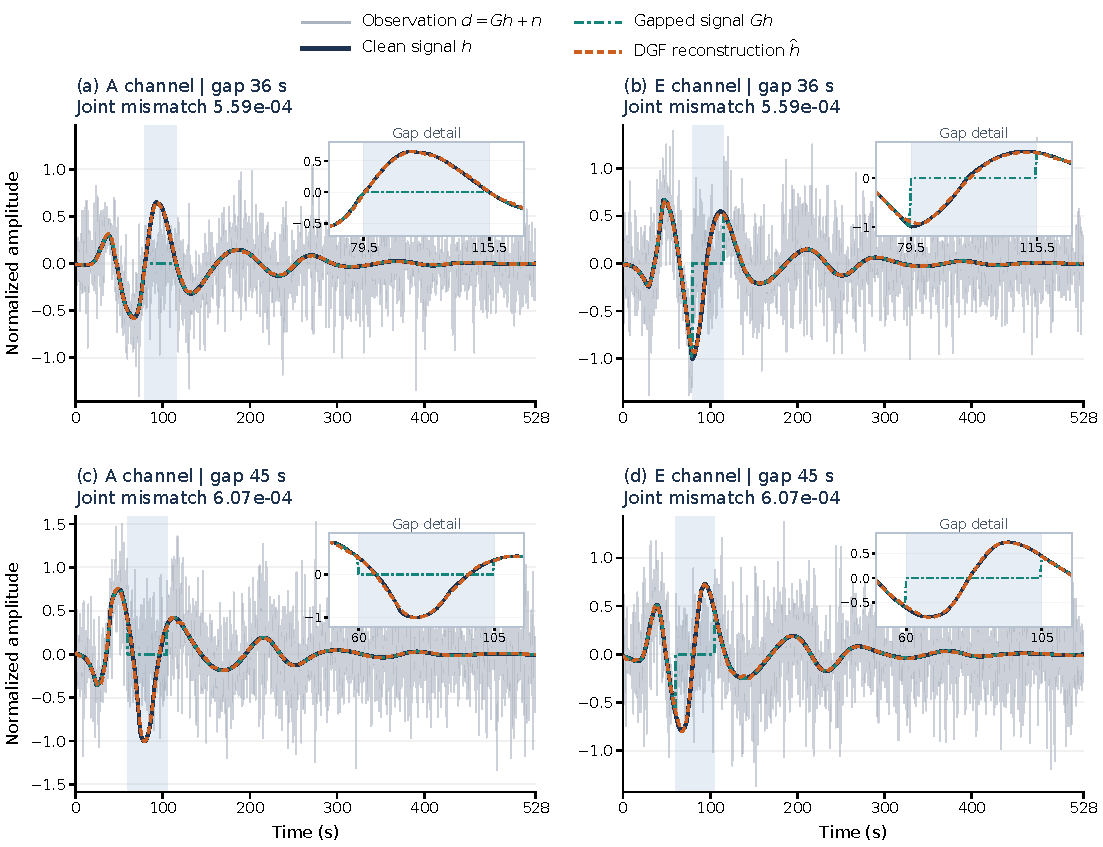
\includegraphics[width=\textwidth]{latest_examples.pdf}
\caption{Waveform reconstruction across 36- and 45-s gaps in the $A$ (left) and $E$ (right) channels. Each panel superposes the noisy observation $d=Gh+n$ (gray), clean signal $h$, gapped clean signal $Gh$ and DGF reconstruction $\widehat h$ over the full 528-s record; insets resolve the gap. Shading marks signal suppression, with noise retained. All four curves use the same clean-signal amplitude normalization per source and connect the original 0.5-s samples. Source seeds, from top to bottom, are 2038202231 and 2038201952. Full-population statistics use all 6,000 test sources.}\label{fig:examples}\end{figure*}

\subsection{Amplitude and spectral fidelity}\label{subsec:MeanSquaredError}\label{subsec:AmplitudeDensityFrequencySpectrum}
Normalized overlap is invariant under positive amplitude rescaling. We therefore evaluate the relative waveform error
\begin{equation}
E=\frac{\left[\sum_{c,j}(\widehat h_{c,j}-h_{c,j})^2\right]^{1/2}}{\left[\sum_{c,j}h_{c,j}^2\right]^{1/2}}.
\end{equation}
Its mean is 0.13424, median 0.10337 and 95th percentile 0.30008. The mean signed norm bias, $\|\widehat h\|_2/\|h\|_2-1$, is -0.01301. Together with mismatch, these measurements characterize waveform shape and overall amplitude fidelity.

For the 1935 sources with envelope peaks inside the gap, the gap-local relative error $\|m(\widehat h-h)\|_2/\|mh\|_2$ has mean 0.13552 and median 0.10337. The denominator measures the clean signal contained within the interval. The full-waveform error $E$ remains the common amplitude-sensitive measure for all sources.

Figure~\ref{fig:psd} compares the mean one-sided periodograms of the reconstruction residual and simulated instrument noise in each channel. Both spectra average all 6,000 test sources and are expressed in fractional-frequency units. They show the frequency dependence of the residual after joint denoising and reconstruction. Mode-resolved frequency and damping-time estimation requires fitting the individual ringdown components.
\begin{figure*}[t]\centering\includegraphics[width=\textwidth]{latest_residual_psd.pdf}
\caption{Mean residual and noise power spectral densities in the $A/E$ channels over all 6,000 test sources. The reconstruction residual is $\widehat h-h$. Fractional-frequency amplitudes are dimensionless, so the PSD has units $\mathrm{Hz}^{-1}$. The curves use the same one-sided periodogram convention.}\label{fig:psd}\end{figure*}

\subsection{Phase recovery}\label{subsec:PhaseRecoveryAlignment}
For each channel, define $z_c=h_c+i\mathcal H[h_c]$ and $\widehat z_c=\widehat h_c+i\mathcal H[\widehat h_c]$. At the clean-signal envelope peak $j_{\star,c}$, the phase error is
\begin{equation}
\Delta\phi_c=\arg[\widehat z_{c,j_{\star,c}}z_{c,j_{\star,c}}^*].
\end{equation}
The mean absolute phase errors are $3.84^\circ$ in $A$ and $3.79^\circ$ in $E$. The corresponding medians are $2.19^\circ$ and $2.14^\circ$, and the 95th percentiles are $12.72^\circ$ and $11.58^\circ$. This diagnostic evaluates the analytic phase of the channel waveform at fixed time; quasinormal-mode phase parameters require a separate mode decomposition.
\begin{figure*}[t]\centering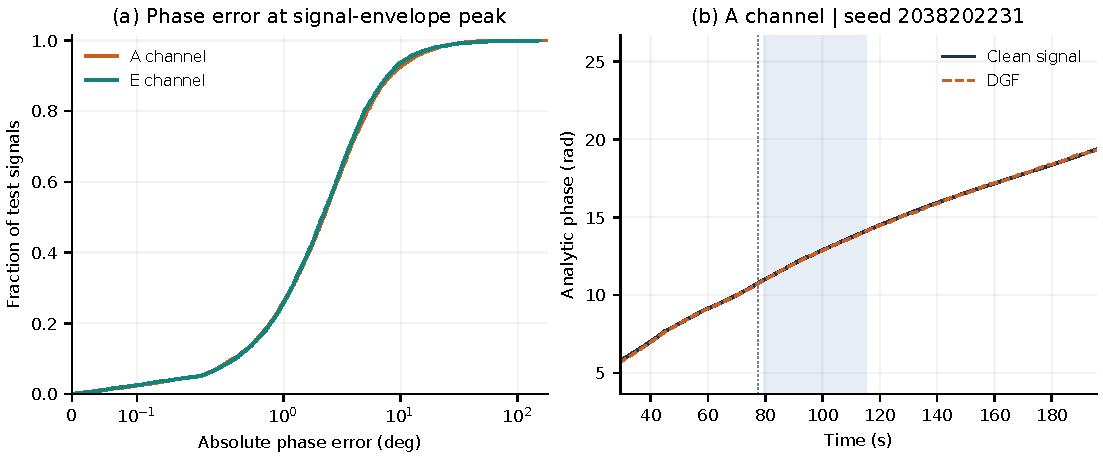
\includegraphics[width=\textwidth]{latest_phase.pdf}
\caption{(a) Absolute phase-error distributions for all 6,000 sources in each channel. (b) Analytic phase of the $A$ channel for source 2038202231, also shown in Fig.~\ref{fig:examples}(a). The displayed clean-signal envelope exceeds 10\% of its peak. The common unwrapped phase branch preserves the relative phase modulo $2\pi$; the arrival time and phase remain fixed. Shading marks the gap and the dotted line marks the clean envelope peak.}\label{fig:phase}\end{figure*}

\section{Discussion and Conclusions}\label{sec:discussion}
We have presented DGF for joint denoising and reconstruction of black hole ringdown signals with data gaps. The network combines complex time--frequency features with signed multiscale temporal information and synthesizes the clean $A/E$ waveforms using the observed context and gap mask. Simulations follow standard LISA response and noise models with the assumptions specified in Sec.~\ref{sec:method}. On the independent variable-gap test, the mean noise-weighted mismatch is 0.00852; the $\rho\ge10$ subset has mean 0.00532. Mean absolute phase errors are $3.84^\circ$ and $3.79^\circ$ in the two channels.

The complete distributions and conditional diagnostics describe the accuracy across the tested source population. In Fig.~\ref{fig:examples}, the gaps contain approximately 43\%--57\% of the signal squared norm, and the reconstructed oscillations follow the clean waveforms across these intervals. The peak-inside-gap subset has mean mismatch 0.00912, compared with 0.00823 for peaks outside the gap. Full-waveform and gap-local residuals quantify amplitude recovery alongside the normalized overlap. The fixed-duration tests in Appendix~\ref{app:fixed_gaps} use the same sources and noise and provide additional checks over the trained gap range.

The simulations cover nonspinning progenitor binaries, isotropic orientations, an idealized equal-arm constellation and stationary Gaussian instrument noise. The analysis uses event-centered 528-s windows and single 32--52-s gaps. The specified pre-reference ring-up fixes the signal history entering the TDI delays; continuous merger histories provide a further robustness test. Extending the model to moving unequal-arm constellations, nonstationary noise, confusion foregrounds, overlapping sources and multiple gaps calls for simulations of those conditions. Reconstruction uncertainty and variation between trained estimators can be assessed with probabilistic models and repeated training runs.

DGF provides a clean-waveform point estimate for waveform inspection and initial estimates in ringdown analysis. Parameter inference uses the original observation likelihood, constructed from $d-Gh(\theta)$ and the noise covariance. Posterior bias and coverage tests would quantify the usefulness of reconstruction in that setting. Bayesian gap treatment~\cite{Baghi2019} and learned denoising~\cite{Wang:2024waveformer} address complementary parts of this analysis. Fitting individual mode frequencies and damping times would connect reconstruction fidelity to black hole spectroscopy.

\begin{acknowledgments}
The authors thank He Wang and Yiyang Guo for helpful discussions. This research is supported in part by the National Key R\&D Program of China, grant number 2020YFC2201300, and the National Natural Science Foundation of China, grant numbers 12035016, 12375058 and 12361141825.

\end{acknowledgments}
\appendix
\section{Implementation and reproducibility}\label{app:model_analysis}
\subsection{Representations and attention}
For each $A/E$ channel, the backbone CWT array has shape $2\times16\times264$, and the temporal patches and fused features have shape $8\times32\times64$. For a feature matrix $Z\in\mathbb R^{32\times64}$, attention is computed as
\begin{equation}
A(Z)=\operatorname{softmax}(ZZ^{\mathsf T}/\sqrt{64})Z.
\end{equation}
Each of the eight feature channels applies this operation, followed by feedforward transformations, residual connections and normalization. The implementation also allocates multihead-attention parameters that are inactive in the forward pass. The quoted total parameter count includes those stored tensors. Attention spans the full sequence.

The db4 representation uses the approximation and seven detail components in library coefficient order. The decoder combines reconstructed patches by overlap averaging and subband summation. Its linear patch map and the encoder embedding map have independent checkpoint values. When loading, we clone the initially transposed storage before reading the tensors so that their saved values are preserved on both CPU and GPU.

\subsection{Numerical and test conventions}
The white-space RMS floor is $10^{-4}$ for coefficient and residual normalization. Training spectral target and prediction squared norms are floored at $10^{-12}$ for finite numerical division, and physical-time relative-error denominators use the same floor in the scaled working representation. Physical evaluation uses float64 transforms, the common frozen PSD and the complete target norm. Overlap is clipped to $[-1,1]$ to bound roundoff. A zero prediction is assigned mismatch one; a zero target triggers a dataset validation failure.

The $A/E$ test seeds are 2038200000--2038205999. The additional fixed-gap training-noise seeds are 2158200000--2158259999. Features are recomputed from each generated observation. The reproducibility record contains raw and EMA checkpoints, training histories, noise calibration, masks, seeds and per-source predictions. SHA-256 manifests identify the source files and fixed assets. Restarting resumes the last completed epoch with its optimizer, scheduler and random-number states.

The simulated response peak determines the event-centered crop and gap metadata. Inference uses the cropped observation, known mask and fixed preprocessing arrays. Clean targets are used in the losses and evaluation. Configurations, source seeds and frozen checkpoint identifiers are included in the evaluation record. The project repository is \url{https://github.com/ljq2088/RingdownGapFilling}.

\section{Additional waveform diagnostics}\label{app:complementary}
Figure~\ref{fig:snr_gap} shows every independent test source as a function of network SNR and separates the distributions by gap location. Both panels use the primary variable-gap predictions from Sec.~\ref{sec:results}. The $\rho\ge10$ summaries retain 5814 of the 6,000 test sources; the complete-population results retain all sources.
\begin{figure*}[t]\centering\includegraphics[width=\textwidth]{latest_snr_gap.pdf}
\caption{Additional diagnostics for the same independent test population. (a) Joint noise-weighted mismatch versus network SNR, with the dotted line at $\rho=10$. (b) Conditional mismatch distributions according to whether the joint signal-envelope peak falls inside the gap. All sources contribute to the complete-population statistics.}\label{fig:snr_gap}\end{figure*}

The two sources in Fig.~\ref{fig:examples} have envelope peaks inside the gap, $\rho\ge10$ and records extending for at least four $\tau_{220}$ after the joint response peak. Their global and gap-local relative errors are below 6\%, and their per-channel peak phase errors are below $2.5^\circ$. The figure data include source seeds, waveform parameters, per-source diagnostics and native-sample curvature used to construct the comparison.



The phase statistics in Sec.~\ref{subsec:PhaseRecoveryAlignment} contain one value per channel and source. This convention preserves source counts when reporting channel-specific means. In intervals containing very little clean signal, gap-local normalization by $\|mh\|_2$ magnifies residuals. The complete-population amplitude diagnostic uses the full target norm, while the main-text gap-local statistic is reported for sources whose joint envelope peaks are inside the interval.


\subsection{Logarithmic amplitude comparison}
Figure~\ref{fig:tdi_log_amplitudes} compares the absolute clean and reconstructed channel amplitudes on a logarithmic scale over the full analysis window. This view resolves the decay and the residuals at small amplitudes. The minima follow the zero crossings of the signed waveforms. The signed comparisons in Fig.~\ref{fig:examples} preserve the accompanying phase information.
\begin{figure*}[t]\centering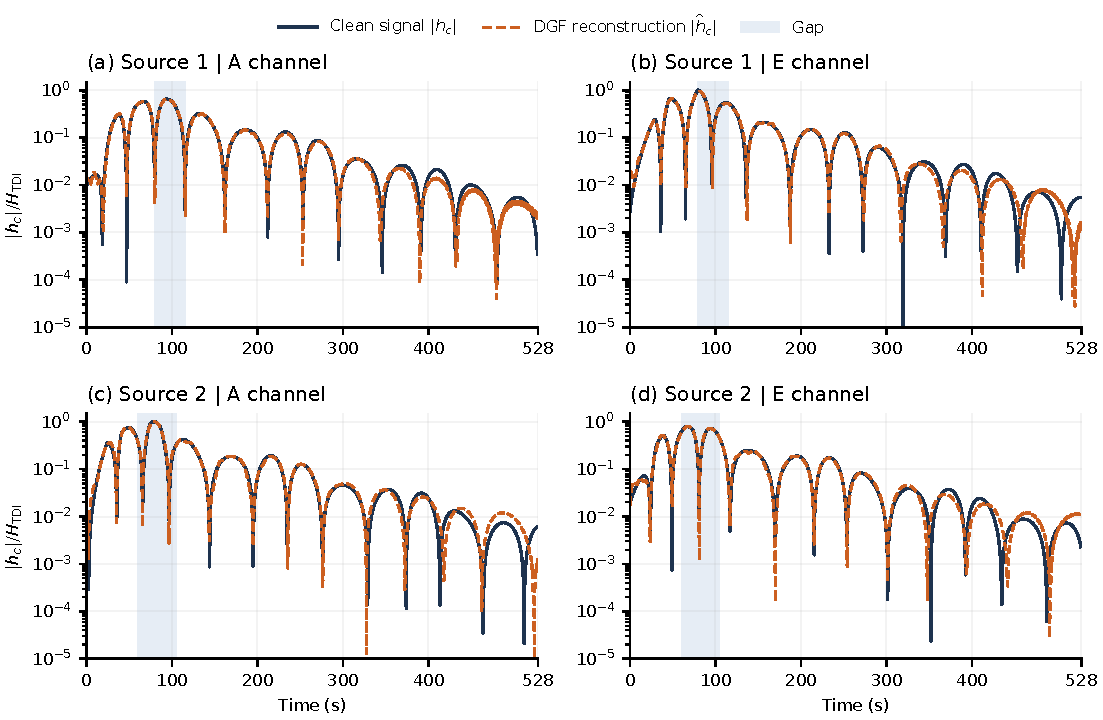
\includegraphics[width=\textwidth]{tdi_log_amplitudes_20261015.pdf}
\caption{Absolute amplitudes of the clean and reconstructed $A$ (left) and $E$ (right) waveforms for the sources in Fig.~\ref{fig:examples}. Each row uses the common scale $H_{\rm TDI}=\max_{c,j}|h_{c,j}|$ from the clean signal. Shading marks the gap. The logarithmic axis resolves small-amplitude structure and differences near zero crossings. All curves use the same physical-time arrays as Fig.~\ref{fig:examples}, with native sampling and fixed arrival time and phase.}\label{fig:tdi_log_amplitudes}
\end{figure*}

\section{Fixed-duration gaps and reference comparison}\label{app:fixed_gaps}
We evaluate 33- and 50-s gaps on the same 6,000 source waveforms and noise realizations, preserving each gap's center. Table~\ref{tab:fixed_gaps} gives the joint noise-weighted mismatch of the selected DGF model. These tests vary the mask while holding the physical source population and noise fixed.
\begin{table}[t]\centering\setlength{\tabcolsep}{2pt}
\caption{Additional gap-duration tests on the same independent sources. Each complete-population row contains 6,000 sources; each $\rho\ge10$ row contains 5814 sources.}\label{tab:fixed_gaps}
\begin{tabular}{lrrr}\hline\hline
Gap and SNR & Mean $\mathcal M_{AE}$ & Median $\mathcal M_{AE}$ & \shortstack{95th\\percentile}\\\hline
33 s / all & 0.00716 & 0.00204 & 0.02389\\
33 s / $\rho\ge10$ & 0.00438 & 0.00195 & 0.01608\\
50 s / all & 0.01112 & 0.00350 & 0.03653\\
50 s / $\rho\ge10$ & 0.00715 & 0.00334 & 0.02498\\
\hline\hline\end{tabular}\end{table}

A reference DGF configuration with joint-channel synthesis and the training-derived signal basis is evaluated on the identical test observations. It uses the preceding fitted synthesis parameters and omits the final noise-conditioned head. For variable gaps, its mean mismatch is 0.00868. The selected model has paired mean difference $-1.61\times10^{-4}$, with 95\% bootstrap interval $[-2.45\times10^{-4},-8.11\times10^{-5}]$. The interval uses 5,000 paired resamples of the independent test sources. This comparison concerns the complete fitted configurations, including their synthesis parameters and coefficient heads.

\clearpage
\bibliography{DGF_references}
\end{document}
